\mainsection{\the\numexpr \thechapter + 1 \relax}{Première structure de contrôle: les tests}{dd/mm/yyyy}

\vspace{-0.8cm}
\section{Introduction}
Sauf mention explicite, les instructions d’un algorithme s’exécutent les unes après les autres, dans l’ordre où elles ont été écrites. Le « chemin » suivi à travers un algorithme est appelé le \textbf{flux d’instructions}, et les constructions qui le modifient sont appelées des \textbf{instructions de contrôle} de flux. On exécute normalement les instructions de la première à la dernière, sauf lorsqu’on rencontre une instruction de contrôle de flux : de telles instructions vont permettre de suivre différents chemins suivant les circonstances. C’est en particulier le cas de l’\textbf{instruction conditionnelle} qui n’exécute une instruction que sous certaines conditions préalables. 

\section{Un exemple}
Par Avec les concepts vus jusqu'ici, un programme exécuté 100 fois de suite donnera 100 fois les mêmes résultats, ce qui présente assez peu d'intérêt. Pour que l'exécution de notre programme dépende de différents paramètres, on utilise des structures de contrôle nommées \textit{instruction conditionnelle}.

La condition est un élément de base d'algorithmique que l'on utilise au quotidien.
\begin{myexample}
	S'il fait beau, j'irai en montagne. 
\end{myexample}
Ces structures permettent d'exécuter ou de ne pas exécuter certaines instructions en fonction de certaines conditions et de changer ainsi le déroulement du programme.


\begin{tabular}{ c  l  }
	Étapes & Instructions \\ \hline
	1 & Se lever  \\ 
	2 & Regarder la météo  \\
	3.1 & S'il fait beau, aller en montagne  \\
\end{tabular}

Un premier moyen d'exprimer des conditions en programmation est l'instruction \textsf{if}. 

\subsection{L'instruction \textsf{if}}
\begin{mydefinition}
	L'instruction \lstinline{if} doit être suivie d'une expression retournant un booléen (\lstinline{True} ou \lstinline{False}) puis d'un symbole \lstinline{:}.  Cette expression peut être une variable contenant un booléen ou une opération retournant un booléen comme les opérateurs \lstinline{<}, \lstinline{>}, \lstinline{==} ou \lstinline{!=}.
\end{mydefinition}

La structure d’une instruction conditionnelle « \lstinline{if} » est la suivante :


\begin{figure}[h!]
	\centering
	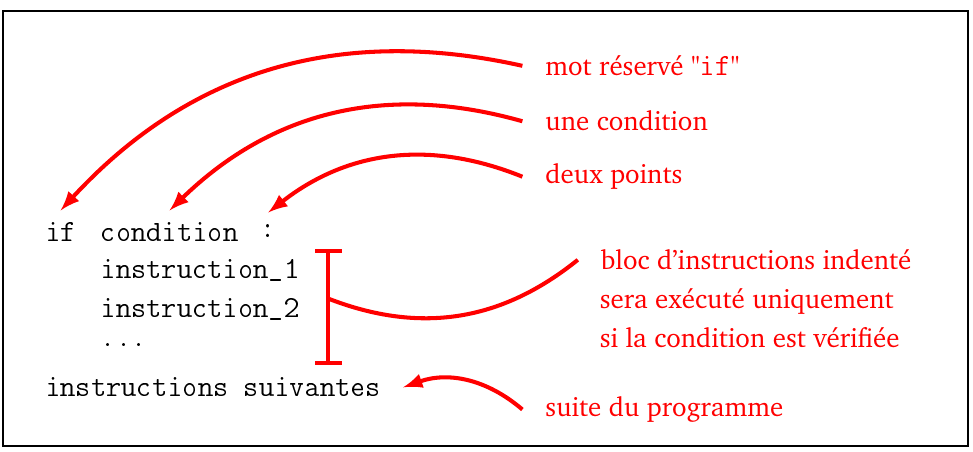
\includegraphics[width=0.7\linewidth]{Images/test/if_structure}
	\caption{Figure tirée du livre \textit{Python au Lycée} de Arnaud Bodin}
\end{figure}


\begin{myexample}
	Un premier moyen d'exprimer des conditions en programmation est l'instruction \textsf{if}. En python, elle s'utilise de la manière suivante : 
	
	\begin{lstlisting}[numbers=none]
if meteo == "beau":
   print("Aujourd'hui, je vais en montagne.")
	\end{lstlisting}
	
	Dans cet exemple, si la variable \lstinline{meteo} a été initialisée à \lstinline{"beau"}, la phrase \lstinline{Aujourd'hui, je vais en montagne.} va s'afficher. Si elle a été initialisée à une autre valeur, par exemple \lstinline{meteo = "moche"}, rien ne s'affichera.
\end{myexample}

%\begin{remarque} Le début et la fin du bloc d'instructions soumis à l'instruction |if| sont définis par l'indentation de chaque ligne (le nombre d'espace avant le début du texte). La condition va s'appliquer à tout le bloc d'instruction suivant qui sera décalé vers la droite par rapport à l'instruction |if|. \end{remarque}

\act
On considère les deux programme suivants:
\begin{multicols}{2}
	\lstset{caption={Programme A}}
	\begin{lstlisting}[numbers=none]
if meteo == "beau":
   print("Aujourd'hui, ")
   print("je vais en montagne.")
	\end{lstlisting}
	
	\lstset{caption={Programme B}}
	\begin{lstlisting}[numbers=none]
if meteo == "beau":
   print("Aujourd'hui, ")
print("je vais en montagne.")
	\end{lstlisting}
\end{multicols}

Remplir le tableau en indiquant ce qu'afficher le programme correspondant en fonction de la valeur de la variable \lstinline{meteo}.

\begin{center}
	\begin{tabular}{p{4cm}|p{6cm}|p{6cm}} 
		& \textbf{Programme A} & \textbf{Programme B}  \\ 
		\hline
		\textbf{Cas 1}\par \lstinline!meteo = "beau"! & \  \par\     \  \par\           &              \\ 
		\hline
		\textbf{Cas 2}\par \lstinline!meteo = "moche"! &    \  \par\   \  \par\            &              \\ 
	\end{tabular}
	\arrayrulecolor{black}
\end{center}
\newpage

\subsection{L'instruction \textsf{else}}
L'instruction \lstinline{if} peut être suivie d'une instruction \lstinline{else} qui est exécutée lorsque le résultat du test est \lstinline{False}. Par exemple, on pourrait préciser la situation précédente :  
\begin{myexample} 
	S'il fait beau, j'irai en montagne. Sinon, j'irai au cinéma. 
\end{myexample}
Notre algorithme deviendrait alors : 
\paragraph{}
\begin{tabular}{ c  l  }
	Étapes & Instructions \\ \hline
	1 & Se lever  \\ 
	2 & Regarder la météo  \\
	3.1 & S'il fait beau, aller en montagne  \\
	3.2 & S'il ne fait pas beau, aller au cinéma  \\
\end{tabular}

\paragraph{}
En python, cela s'écrirait de la manière suivante :

\lstset{caption={Instruction \lstinline{if} - \lstinline{else}}}
\begin{lstlisting}[numbers=none]
if meteo == "beau":
   print("Aujourd'hui, je vais en montagne.")
else:
   print("Aujourd'hui, je vais au cinéma.")
\end{lstlisting}

La structure complète d'une instruction conditionnelle avec un bloc "sinon" est la suivante:
% TODO: \usepackage{graphicx} required
\begin{figure}[h!]
	\centering
	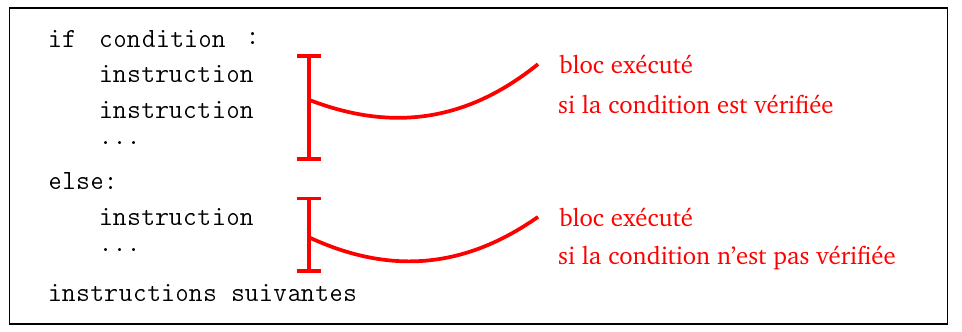
\includegraphics[width=0.7\linewidth]{Images/test/if_else_structure}
	\caption{Figure tirée du livre \textit{Python au Lycée} de Arnaud Bodin}
	\label{fig:ifelsestructure}
\end{figure}

\newpage
\subsection{L'instruction \textsf{elif}}
Dans le cas d'une situation non binaire, on peut introduire des conditions supplémentaires qui sont examinées si les conditions précédentes ne sont pas remplies. On peut par exemple nuancer notre situation ainsi : 

\begin{myexample} 
	S'il fait beau, j'irai en montagne. S'il ne fait pas beau et qu'il pleut, j'irai au cinéma. Sinon, j'irai courir au bord du Rhône. 
\end{myexample}

\begin{myremarque} 
	Ici, le terme \textit{Sinon} signifie "S'il ne fait pas beau et qu'il ne pleut pas". C'est pareil en python, l'instruction conditionnée par \lstinline{else} est exécutée si toutes les conditions précédentes sont fausses.
\end{myremarque}


Notre algorithme devient alors : 

\begin{tabular}{ c  l  }
	Étapes & Instructions \\ \hline
	1 & Se lever  \\ 
	2 & Regarder la météo  \\
	3.1 & S'il fait beau, aller en montagne  \\
	3.2 & S'il ne fait pas beau et qu'il pleut, aller au cinéma  \\
	3.3 & S'il ne fait pas beau et qu'il pleut pas, aller courir au bord du Rhône \\
\end{tabular}


En python, on utilise l'instruction \lstinline{elif} qui est la contraction de "\lstinline{else if}" :

\lstset{caption={Instruction if - else}}
\begin{lstlisting}[numbers=none]
if meteo == "beau":
   print("Aujourd'hui, je vais en montagne.")
elif meteo == "pluie":
   print("Aujourd'hui, je vais au cinéma.")
else:
   print("Aujourd'hui, je vais courir au bord du Rhône.")
\end{lstlisting}
